% ============================================================
%  ОТЧЁТ
%  Лабораторная работа №1
%  Дисциплина: Информационно-поисковые системы
%  РУДН, 2025
% ============================================================

\documentclass[12pt, a4paper]{report}

% ── Кодировки и язык ────────────────────────────────────────
\usepackage[utf8]{inputenc}
\usepackage[T2A]{fontenc}
\usepackage[russian, english]{babel}

% ── Геометрия страницы (ГОСТ 7.32) ──────────────────────────
\usepackage[
  left   = 30mm,
  right  = 15mm,
  top    = 20mm,
  bottom = 20mm
]{geometry}

% ── Шрифты ──────────────────────────────────────────────────
\usepackage{mathptmx}          % Times New Roman (основной текст)
\usepackage{helvet}            % Helvetica (заголовки)
\usepackage[scaled=0.85]{beramono} % моноширинный шрифт

% ── Межстрочный интервал и отступы ──────────────────────────
\usepackage{setspace}
\setstretch{1.5}               % полуторный интервал (ГОСТ)

\usepackage{indentfirst}
\setlength{\parindent}{1.25cm}
\setlength{\parskip}{0pt}

% ── Заголовки разделов ───────────────────────────────────────
\usepackage{titlesec}

\titleformat{\chapter}[block]
  {\sffamily\Large\bfseries\color{NavyBlue}}
  {\thechapter.}{0.5em}{}
\titlespacing{\chapter}{0pt}{12pt}{8pt}

\titleformat{\section}[block]
  {\sffamily\large\bfseries\color{SteelBlue}}
  {\thesection.}{0.5em}{}
\titlespacing{\section}{0pt}{10pt}{6pt}

\titleformat{\subsection}[block]
  {\sffamily\normalsize\bfseries\color{SteelBlue!80!black}}
  {\thesubsection.}{0.5em}{}
\titlespacing{\subsection}{0pt}{8pt}{4pt}

% ── Цвета ────────────────────────────────────────────────────
\usepackage[dvipsnames, table]{xcolor}
\definecolor{NavyBlue}   {RGB}{31,  78, 121}
\definecolor{SteelBlue}  {RGB}{46, 117, 182}
\definecolor{LightBlue}  {RGB}{222,234,246}
\definecolor{PlaceholderBg}{RGB}{255,251,230}
\definecolor{PlaceholderBorder}{RGB}{200,180,120}
\definecolor{CodeBg}     {RGB}{245,245,245}
\definecolor{CodeBorder} {RGB}{46, 117, 182}

% ── Таблицы ─────────────────────────────────────────────────
\usepackage{booktabs}
\usepackage{tabularx}
\usepackage{multirow}
\usepackage{longtable}
\usepackage{array}
\renewcommand{\arraystretch}{1.4}

% ── Листинги кода ────────────────────────────────────────────
\usepackage{listings}
\lstset{
  language        = Python,
  basicstyle      = \ttfamily\small,
  keywordstyle    = \bfseries\color{NavyBlue},
  commentstyle    = \itshape\color{gray},
  stringstyle     = \color{SteelBlue!80!black},
  backgroundcolor = \color{CodeBg},
  frame           = leftline,
  framerule       = 2pt,
  rulecolor       = \color{CodeBorder},
  numbers         = left,
  numberstyle     = \tiny\color{gray},
  numbersep       = 8pt,
  showstringspaces= false,
  breaklines      = true,
  breakatwhitespace= true,
  inputencoding   = utf8,
  extendedchars   = true,
  literate        = % поддержка кириллицы в lstlisting
    {а}{{\cyra}}1 {б}{{\cyrb}}1 {в}{{\cyrv}}1 {г}{{\cyrg}}1
    {д}{{\cyrd}}1 {е}{{\cyre}}1 {ё}{{\cyryo}}1 {ж}{{\cyrzh}}1 {з}{{\cyrz}}1
    {и}{{\cyri}}1 {й}{{\cyrishrt}}1 {к}{{\cyrk}}1 {л}{{\cyrl}}1
    {м}{{\cyrm}}1 {н}{{\cyrn}}1 {о}{{\cyro}}1 {п}{{\cyrp}}1
    {р}{{\cyrr}}1 {с}{{\cyrs}}1 {т}{{\cyrt}}1 {у}{{\cyru}}1
    {ф}{{\cyrf}}1 {х}{{\cyrh}}1 {ц}{{\cyrc}}1 {ч}{{\cyrch}}1
    {ш}{{\cyrsh}}1 {щ}{{\cyrshch}}1 {ъ}{{\cyrhrdsn}}1 {ы}{{\cyrery}}1
    {ь}{{\cyrsftsn}}1 {э}{{\cyrerev}}1 {ю}{{\cyryu}}1 {я}{{\cyrya}}1
    {А}{{\CYRA}}1 {Б}{{\CYRB}}1 {В}{{\CYRV}}1 {Г}{{\CYRG}}1
    {Д}{{\CYRD}}1 {Е}{{\CYRE}}1 {Ж}{{\CYRZH}}1 {З}{{\CYRZ}}1
    {И}{{\CYRI}}1 {К}{{\CYRK}}1 {Л}{{\CYRL}}1 {М}{{\CYRM}}1
    {Н}{{\CYRN}}1 {О}{{\CYRO}}1 {П}{{\CYRP}}1 {Р}{{\CYRR}}1
    {С}{{\CYRS}}1 {Т}{{\CYRT}}1 {У}{{\CYRU}}1 {Ф}{{\CYRF}}1
    {Х}{{\CYRH}}1 {Ц}{{\CYRC}}1 {Ч}{{\CYRCH}}1 {Ш}{{\CYRSH}}1
    {Щ}{{\CYRSHCH}}1 {Ъ}{{\CYRHRDSN}}1 {Ы}{{\CYRERY}}1 {Ь}{{\CYRSFTSN}}1
    {Э}{{\CYREREV}}1 {Ю}{{\CYRYU}}1 {Я}{{\CYRYA}}1,
  captionpos      = b,
  xleftmargin     = 1.25cm,
}

% ── Рамки и боксы ────────────────────────────────────────────
\usepackage{tcolorbox}
\tcbuselibrary{skins, breakable}

% Рамка-заполнитель (placeholder)
\tcbset{
  placeholderbox/.style = {
    colback    = PlaceholderBg,
    colframe   = PlaceholderBorder,
    fonttitle  = \sffamily\small\bfseries,
    fontupper  = \itshape\small\color{gray!60!black},
    boxrule    = 0.6pt,
    left       = 6pt, right = 6pt,
    top        = 4pt, bottom= 4pt,
    breakable,
    before upper = {},
  },
  infobox/.style = {
    colback  = LightBlue,
    colframe = NavyBlue,
    fonttitle= \sffamily\small\bfseries\color{NavyBlue},
    boxrule  = 1pt,
    left     = 8pt, right = 8pt,
    top      = 6pt, bottom= 6pt,
    breakable,
  },
}

\newcommand{\placeholder}[2][Вставьте результат]{%
  \begin{tcolorbox}[placeholderbox, title={#2}]
    #1
  \end{tcolorbox}%
  \vspace{4pt}%
}

% ── Прочие пакеты ────────────────────────────────────────────
\usepackage{graphicx}
\usepackage{subcaption}
\usepackage{caption}
\captionsetup{font=small, labelfont={bf,sf}, labelsep=period}

\usepackage{enumitem}
\setlist[enumerate]{leftmargin=1.5cm, itemsep=2pt, parsep=0pt}
\setlist[itemize]  {leftmargin=1.5cm, itemsep=2pt, parsep=0pt}

\usepackage{hyperref}
\hypersetup{
  colorlinks = true,
  linkcolor  = NavyBlue,
  urlcolor   = SteelBlue,
  citecolor  = NavyBlue,
  pdftitle   = {Отчёт ЛР №1 — Информационно-поисковые системы},
}

\usepackage{fancyhdr}
\usepackage{lastpage}
\usepackage{amsmath}
\usepackage{microtype}

% ── Колонтитулы ──────────────────────────────────────────────
\pagestyle{fancy}
\fancyhf{}
\fancyhead[R]{\sffamily\footnotesize\color{gray}Лабораторная работа №1\ |\ Информационно-поисковые системы}
\fancyfoot[C]{\sffamily\footnotesize\color{gray}\thepage\ из\ \pageref{LastPage}}
\renewcommand{\headrulewidth}{0.4pt}
\renewcommand{\footrulewidth}{0.4pt}
\renewcommand{\headrule}{\color{SteelBlue}\hrule width\headwidth height\headrulewidth}
\renewcommand{\footrule}{\color{SteelBlue}\hrule width\headwidth height\footrulewidth}

% ── Подавление колонтитулов на chapter-страницах ─────────────
\fancypagestyle{plain}{%
  \fancyhf{}
  \fancyfoot[C]{\sffamily\footnotesize\color{gray}\thepage\ из\ \pageref{LastPage}}
  \renewcommand{\headrulewidth}{0pt}
  \renewcommand{\footrulewidth}{0.4pt}
  \renewcommand{\footrule}{\color{SteelBlue}\hrule width\headwidth height\footrulewidth}
}

% ── Нумерация глав без слова «Глава» ─────────────────────────
\renewcommand{\chaptername}{}

% ============================================================
\begin{document}
\setcounter{chapter}{0}

% ── Титульная страница ────────────────────────────────────────
\begin{titlepage}
\thispagestyle{empty}
\begin{center}

  {\sffamily\small\bfseries МИНИСТЕРСТВО НАУКИ И ВЫСШЕГО ОБРАЗОВАНИЯ\\
  РОССИЙСКОЙ ФЕДЕРАЦИИ}

  \vspace{6pt}
  {\sffamily\small\bfseries ФЕДЕРАЛЬНОЕ ГОСУДАРСТВЕННОЕ АВТОНОМНОЕ\\
  ОБРАЗОВАТЕЛЬНОЕ УЧРЕЖДЕНИЕ ВЫСШЕГО ОБРАЗОВАНИЯ}

  \vspace{8pt}
  {\sffamily\normalsize\bfseries
 <<МОСКОВСКИЙ ГОСУДАРСТВЕННЫЙ ТЕХНИЧЕСКИЙ УНИВЕРСИТЕТ ИМЕНИ Н.Э.~БАУМАНА (НАЦИОНАЛЬНЫЙ ИССЛЕДОВАТЕЛЬСКИЙ УНИВЕРСИТЕТ)>>}

  \vspace{6pt}
  {\sffamily\small Факультет \underline{Информатика и системы управления}}\\[2pt]
  {\sffamily\small Кафедра \underline{Программное обеспечение ЭВМ и информационные технологии}}

  \vspace{10pt}
  \textcolor{SteelBlue}{\rule{\linewidth}{1pt}}
  \vspace{12pt}

  {\sffamily\Large\bfseries\color{NavyBlue}
  ИНФОРМАЦИОННО-ПОИСКОВЫЕ СИСТЕМЫ}

  \vspace{20pt}

  {\sffamily\LARGE\bfseries ОТЧЁТ}\\[6pt]
  {\sffamily\large по лабораторной работе №1}

  \vspace{12pt}
  \begin{tcolorbox}[infobox, title={}]
    \centering\sffamily\large\bfseries\color{NavyBlue}
    Предобработка текстовых данных\\
    для анализа судебных документов
  \end{tcolorbox}

  \vspace{10pt}

\end{center}

% Таблица данных студента
\begin{flushright}
	\begin{tabular}{p{5cm}p{7cm}}
		\toprule
		\rowcolor{LightBlue}
		\sffamily\small\bfseries Поле & \sffamily\small\bfseries Значение \\
		\midrule
		\sffamily\small Студент       & \underline{Сапожков~А.М.\hspace{3.5cm}} \\[4pt]
		\sffamily\small Группа        & \underline{ИУ7-43М\hspace{4.5cm}} \\[4pt]
		\sffamily\small Специальность & \underline{Программная инженерия\hspace{1.5cm}} \\[4pt]
		\sffamily\small Преподаватель & \underline{Курашкин~С.О.\hspace{3.5cm}} \\[4pt]
		\sffamily\small Дата сдачи    & \underline{\hspace{6.5cm}} \\[4pt]
		\sffamily\small Оценка        & \underline{\hspace{6.5cm}} \\
		\bottomrule
	\end{tabular}
\end{flushright}

\vfill
\begin{center}
  {\sffamily\normalsize Москва, 2026}
\end{center}
\end{titlepage}

% ── Оглавление ───────────────────────────────────────────────
\tableofcontents
\thispagestyle{plain}
\clearpage

% ============================================================
%  РАЗДЕЛ 1. ЦЕЛЬ И ЗАДАЧИ
% ============================================================
\chapter{Цель и задачи работы}

Целью настоящей лабораторной работы является освоение методов предобработки
текстовых данных применительно к корпусу судебных документов, а также формирование
практических навыков применения инструментов обработки естественного языка (NLP)
на языке программирования Python.

В ходе выполнения работы студент решает следующие задачи:

\begin{enumerate}
  \item Формирование и первичный анализ учебного корпуса судебных актов.
  \item Реализация конвейера очистки текстовых данных.
  \item Токенизация, нормализация регистра и фильтрация стоп-слов.
  \item Морфологическая нормализация (лемматизация) с применением библиотеки \texttt{pymorphy2}.
  \item Извлечение именованных сущностей (NER) с применением библиотеки \texttt{natasha}.
  \item Реализация ключевое-словарного классификатора документов.
  \item Количественный анализ корпуса и визуализация результатов.
\end{enumerate}

% ============================================================
%  РАЗДЕЛ 2. ТЕОРЕТИЧЕСКАЯ СПРАВКА
% ============================================================
\chapter{Краткая теоретическая справка}

\begin{tcolorbox}[infobox, title={Источники}]
  Подробное изложение теоретического материала представлено в конспектах Лекции 1
  («Введение в информационно-аналитические системы в юридической практике»)
  и Лекции 2 («Сбор и предобработка данных для анализа судебной практики»).
\end{tcolorbox}

\vspace{8pt}

\section{Предобработка текстовых данных}

Предобработка данных представляет собой совокупность методов, приводящих исходный
неструктурированный текст в форму, пригодную для применения алгоритмов машинного обучения.
Качество предобработки напрямую определяет качество последующей аналитики: неудалённые
артефакты форматирования, нелемматизированные словоформы или сохранённые стоп-слова снижают
точность моделей классификации~\cite{lec2}.

\section{Ключевые операции NLP-конвейера}

\textbf{Токенизация} — процесс разбиения текста на минимальные смысловые единицы (токены).
Является обязательным первым шагом любого NLP-конвейера.

\textbf{Лемматизация} — приведение слова к его нормальной словарной форме с учётом
морфологических свойств. Для русскоязычных текстов применяется библиотека \texttt{pymorphy2},
обеспечивающая морфологический анализ на основе словарей OpenCorpora.

\textbf{Стоп-слова} — частотные служебные слова (предлоги, союзы, местоимения),
не несущие самостоятельного смысла и удаляемые при анализе текста.

\textbf{Распознавание именованных сущностей} (NER, Named Entity Recognition) —
задача выделения из текста упоминаний объектов реального мира (персон, организаций,
дат) и их классификации по типам~\cite{lec1}. В данной работе используется библиотека
\texttt{natasha}, специализированная для обработки русскоязычных текстов.

% ============================================================
%  РАЗДЕЛ 3. ХОД ВЫПОЛНЕНИЯ
% ============================================================
\chapter{Ход выполнения работы}

\section{Анализ корпуса (Задание 1.1)}

В ходе первичного анализа учебного корпуса были получены результаты по количеству документов и
среднему объёму текста по категориям.

\begin{table}[h]
  \centering
  \caption{Результаты анализа корпуса судебных документов}
  \label{tab:corpus_analysis}
  \rowcolors{2}{LightBlue!40}{white}
  \begin{tabularx}{0.9\textwidth}{l X X}
    \toprule
    \rowcolor{LightBlue}
    \textsf{\textbf{Категория}} &
    \textsf{\textbf{Количество документов}} &
    \textsf{\textbf{Средний объём (символы)}} \\
    \midrule
    Оспаривание сделок должника & 3 & 568.3 \\
    Субсидиарная ответственность & 3 & 494.0 \\
    Обжалование налоговых решений & 2 & 564.5 \\
    Включение в реестр требований кредиторов & 2 & 494.0 \\
    \midrule
    \textbf{Итого} & \textbf{10} & \textbf{530.2 (среднее)} \\
    \bottomrule
  \end{tabularx}
\end{table}

% ── 3.2 ─────────────────────────────────────────────────────
\section{Очистка текста (Задания 2.1–2.2)}

Были реализованы функции очистки текста. Ниже приведён исходный код и пояснения к каждому шагу.

\begin{lstlisting}[caption={Реализация функций очистки текста}, label={lst:cleaning}]
def normalize_whitespace(text: str) -> str:
    """Нормализует пробельные символы."""
    # Заменяем все последовательности пробельных символов (\s+) 
    # на единственный пробел, удаляем пробелы в начале и конце
    text = re.sub(r'\s+', ' ', text).strip()
    return text


def remove_punctuation(text: str) -> str:
    """Удаляет знаки пунктуации, сохраняя дефисы внутри слов."""
    # Сначала заменяем дефисы-разделители (не находящиеся между буквами)
    # на пробел, затем удаляем оставшуюся пунктуацию
    text = re.sub(r'(?<![а-яА-Яa-zA-Z])-(?![а-яА-Яa-zA-Z])', ' ', text)
    text = text.translate(str.maketrans('', '', string.punctuation))
    return text


def clean_text(text: str) -> str:
    """Полный конвейер очистки текста."""
    text = remove_html_tags(text)
    text = remove_special_chars(text)
    text = normalize_whitespace(text)
    return text.lower()
\end{lstlisting}

\begin{table}[h]
  \centering
  \caption{Пример результата очистки текста}
  \label{tab:cleaning_example}
  \begin{tabularx}{\textwidth}{@{}l X@{}}
    \toprule
    \rowcolor{LightBlue}
    \textsf{\textbf{Этап}} & \textsf{\textbf{Текст (фрагмент)}} \\
    \midrule
    Исходный текст & 
    Арбитражный суд г. Москвы рассмотрел заявление конкурсного управляющего ООО 'Строй-Инвест' Иванова А.П. о признании недействительной сделки — договора купли-продажи... \\
    \midrule
    После очистки & 
    арбитражный суд г. москвы рассмотрел заявление конкурсного управляющего ооо 'строй-инвест' иванова а.п. о признании недействительной сделки договора купли-продажи... \\
    \bottomrule
  \end{tabularx}
\end{table}

% ── 3.3 ─────────────────────────────────────────────────────
\section{Токенизация и удаление стоп-слов (Задания 3.1–3.2)}

Было проведено обоснование выбора дополнительных юридических стоп-слов. Ниже приведены результаты токенизации.

\begin{tcolorbox}[infobox, title={Дополнительные юридические стоп-слова}]
В дополнение к базовому набору стоп-слов NLTK были добавлены следующие юридические термины:

\textbf{Процессуальные термины:} суд, суда, судебный, арбитражный, решение, решения, дело, дела, заявление, заявления, рассмотрение, рассмотрев, установил, установлено, признал, признать, удовлетворить, удовлетворено, отказать, отказано.

\textbf{Ролевые обозначения:} истец, истца, ответчик, ответчика, заявитель, заявителя, кредитор, кредитора, должник, должника, управляющий, управляющего.

\textbf{Документы и акты:} договор, договора, контракт, контракта, акт, акта, протокол, протокола.

\textbf{Временные и указательные слова:} дата, даты, момент, момента, период, периода, год, года, году, лет, число, числа, настоящий, данного, данный, который, которого, такой, такого.

\textbf{Прочие часто встречающиеся слова:} право, права, закону, закон, статья, статьи, статье, ст, пункт, пункта, пункту, п, часть, части, частью, основание, основания, основанию, порядок, порядка, порядку.

\textbf{Обоснование:} Данные слова встречаются в большинстве судебных актов независимо от их категории и не несут дифференцирующей информации для задач классификации. Их удаление позволяет алгоритму фокусироваться на содержательных терминах, специфичных для каждой категории дел.
\end{tcolorbox}

\begin{table}[h]
  \centering
  \caption{Пример токенизации документа A40-001-2023}
  \label{tab:tokenization_example}
  \begin{tabularx}{\textwidth}{@{}l X@{}}
    \toprule
    \rowcolor{LightBlue}
    \textsf{\textbf{Параметр}} & \textsf{\textbf{Значение}} \\
    \midrule
    Документ & A40-001-2023 \\
    Категория & Оспаривание сделок должника \\
    Первые 15 токенов & ['москвы', 'конкурсного', 'ооо', 'иванова', 'признании', 'недействительной', 'сделки', 'нежилых', 'помещений', 'заключённого', 'ооо', 'соответствии', 'федерального', 'несостоятельности', 'банкротстве'] \\
    \bottomrule
  \end{tabularx}
\end{table}

% ── 3.4 ─────────────────────────────────────────────────────
\section{Лемматизация (Задания 4.1–4.2)}

Была реализована функция \texttt{lemmatize\_tokens}. Продемонстрировано, что
лемматизация объединяет словоформы одного слова.

\begin{lstlisting}[caption={Реализация функции лемматизации}, label={lst:lemmatization}]
morph = pymorphy2.MorphAnalyzer()

def lemmatize_tokens(tokens: list) -> list:
    """
    Приводит список токенов к нормальной форме с помощью pymorphy2.
    Возвращает список лемм.
    """
    lemmas = []
    for token in tokens:
        lemma = morph.parse(token)[0].normal_form
        lemmas.append(lemma)
    return lemmas
\end{lstlisting}

Для наглядности проведено сравнение частотных словарей до и после лемматизации. Пример оформления
представлен в таблице~\ref{tab:lemma_compare}. Таблица заполнена данными из первого документа корпуса.

\begin{table}[h]
  \centering
  \caption{Сравнение частотных словарей до и после лемматизации (топ-10)}
  \label{tab:lemma_compare}
  \rowcolors{2}{LightBlue!40}{white}
  \begin{tabularx}{0.9\textwidth}{c X c X c}
    \toprule
    \rowcolor{LightBlue}
    \textsf{\textbf{\#}} &
    \textsf{\textbf{Токен}} &
    \textsf{\textbf{Частота}} &
    \textsf{\textbf{Лемма}} &
    \textsf{\textbf{Частота}} \\
    \midrule
    1  & москвы & 1 & москва & 1 \\
    2  & конкурсного & 1 & конкурсый & 1 \\
    3  & ооо & 2 & ооо & 2 \\
    4  & иванова & 1 & иванов & 1 \\
    5  & признании & 1 & признание & 1 \\
    6  & недействительной & 1 & недействительный & 1 \\
    7  & сделки & 1 & сделка & 1 \\
    8  & нежилых & 1 & нежилой & 1 \\
    9  & помещений & 1 & помещение & 1 \\
    10 & заключённого & 1 & заключить & 1 \\
    \bottomrule
  \end{tabularx}
\end{table}

% ── 3.5 ─────────────────────────────────────────────────────
\section{Извлечение именованных сущностей (Задания 5.1–5.2)}

Были получены результаты работы NER-модуля. Ниже приведены наблюдения относительно точности.

\begin{table}[h]
  \centering
  \caption{Именованные сущности в документе A40-001-2023}
  \label{tab:ner_example}
  \rowcolors{2}{LightBlue!40}{white}
  \begin{tabularx}{0.7\textwidth}{l X}
    \toprule
    \rowcolor{LightBlue}
    \textsf{\textbf{Тип}} & \textsf{\textbf{Сущность}} \\
    \midrule
    ORG & Арбитражный суд \\
    LOC & Москвы \\
    ORG & ООО 'Строй-Инвест' \\
    PER & Иванова А.П. \\
    ORG & ООО 'Партнёр' \\
    \bottomrule
  \end{tabularx}
\end{table}

\begin{table}[h]
  \centering
  \caption{Сводная таблица именованных сущностей по корпусу}
  \label{tab:ner_summary}
  \rowcolors{2}{LightBlue!40}{white}
  \begin{tabularx}{0.9\textwidth}{c X c X}
    \toprule
    \rowcolor{LightBlue}
    \multicolumn{2}{c}{\textsf{\textbf{Организации (ORG)}}} &
    \multicolumn{2}{c}{\textsf{\textbf{Персоны (PER)}}} \\
    \cmidrule(r){1-2} \cmidrule(l){3-4}
    \textsf{\textbf{Название}} & \textsf{\textbf{Частота}} & \textsf{\textbf{ФИО}} & \textsf{\textbf{Частота}} \\
    \midrule
    Арбитражный суд & 5 & Иванова А.П. & 1 \\
    ООО 'Партнёр' & 2 & Петрова Д.С. & 1 \\
    ООО 'Строй-Инвест' & 1 & Сидоровым В.И. & 1 \\
    Арбитражного суда & 1 & Сидоровой О.Н & 1 \\
    ЗАО 'Балтик Трейд' & 1 & Кузнецова М.В & 1 \\
    \bottomrule
  \end{tabularx}
\end{table}

\begin{tcolorbox}[infobox, title={Наблюдения по работе NER}]
\textbf{Распознаваемые типы сущностей:}
\begin{itemize}
  \item \textbf{ORG} — Организации (ООО, ПАО, ЗАО, Арбитражный суд)
  \item \textbf{PER} — Персоны (люди с фамилией и инициалами)
  \item \textbf{LOC} — Локации (города, области)
\end{itemize}

\textbf{Хорошо распознаются:}
\begin{itemize}
  \item Организации с чёткой формой: ООО, ПАО, ЗАО + название в кавычках
  \item Судебные органы: «Арбитражный суд» определяется как ORG
  \item Персоны с фамилией и инициалами (Фамилия И.О.)
  \item Географические названия (города, области)
\end{itemize}

\textbf{Возможные ошибки/ограничения:}
\begin{itemize}
  \item Дублирование сущностей — одна и та же организация может быть извлечена несколько раз
  \item Частичное извлечение названий — «Арбитражный суд» без указания города/региона
  \item Физические лица без инициалов могут не определяться как PER
  \item Государственные органы (ИФНС, налоговая служба) могут определяться не всегда корректно
\end{itemize}
\end{tcolorbox}

% ── 3.6 ─────────────────────────────────────────────────────
\section{Ключевое-словарная классификация (Задания 6.1–6.2)}

Описан принцип работы реализованного классификатора. Указаны леммы, добавленные в словарь, и основания для их добавления.

\begin{lstlisting}[caption={Расширенный словарь ключевых лемм}, label={lst:keywords}]
KEYWORD_DICT = {
    "Оспаривание сделок должника": [
        "сделка", "недействительный", "оспаривание",
        "подозрительный", "предпочтение", "зачёт",
        "договор", "купля", "продажа", "дарение",
        "ущерб", "кредитор", "имуществ", "возврат",
        "стоимость", "цена", "неплатёжеспособность"
    ],
    "Субсидиарная ответственность": [
        "субсидиарный", "ответственность", "контролировать",
        "генеральный", "директор", "довести",
        "банкротство", "актив", "вывод", "аффилированный",
        "структура", "взыскать", "задолженность", "солидарный",
        "участник", "директор", "управляющий", "документация"
    ],
    "Обжалование налоговых решений": [
        "налог", "доначисление", "вычет",
        "ифнс", "налогоплательщик", "трансфертный",
        "прибыль", "ндс", "добавленный", "стоимость",
        "контрагент", "технический", "компания", "хозяйственный",
        "операция", "доказательство", "налоговый"
    ],
    "Включение в реестр требований кредиторов": [
        "реестр", "требование", "кредитор",
        "очередь", "включение", "банк",
        "задолженность", "кредит", "договор", "залог",
        "обеспеченный", "третий", "отказать", "удовлетворить",
        "заявление", "основание", "корпоративный", "заём"
    ]
}
\end{lstlisting}

Результаты классификации представлены в таблице~\ref{tab:classification}.

\begin{table}[h]
  \centering
  \caption{Результаты ключевое-словарной классификации документов}
  \label{tab:classification}
  \rowcolors{2}{LightBlue!30}{white}
  \begin{tabularx}{\textwidth}{l X X c}
    \toprule
    \rowcolor{LightBlue}
    \textsf{\textbf{ID документа}} &
    \textsf{\textbf{Истинная категория}} &
    \textsf{\textbf{Предсказанная категория}} &
    \textsf{\textbf{Верно}} \\
    \midrule
    A40-001-2023 & Оспаривание сделок должника & Оспаривание сделок должника & Да \\
    A40-002-2023 & Оспаривание сделок должника & Оспаривание сделок должника & Да \\
    A56-003-2023 & Субсидиарная ответственность & Субсидиарная ответственность & Да \\
    A56-004-2023 & Субсидиарная ответственность & Субсидиарная ответственность & Да \\
    A60-005-2023 & Обжалование налоговых решений & Обжалование налоговых решений & Да \\
    A60-006-2023 & Обжалование налоговых решений & Обжалование налоговых решений & Да \\
    A07-007-2023 & Включение в реестр требований кредиторов & Включение в реестр требований кредиторов & Да \\
    A07-008-2023 & Включение в реестр требований кредиторов & Включение в реестр требований кредиторов & Да \\
    A40-009-2023 & Оспаривание сделок должника & Оспаривание сделок должника & Да \\
    A40-010-2023 & Субсидиарная ответственность & Субсидиарная ответственность & Да \\
    \midrule
    \multicolumn{3}{r}{\textsf{\textbf{Точность}}} & \textbf{10/10 = 100.0\%} \\
    \bottomrule
  \end{tabularx}
\end{table}

% ── 3.7 ─────────────────────────────────────────────────────
\section{Визуализация результатов (Задания 7.1–7.3)}

Были построены графики и облака слов. Каждый рисунок сопровождается
подписью и пояснительным текстом.

\begin{figure}[h]
  \centering
  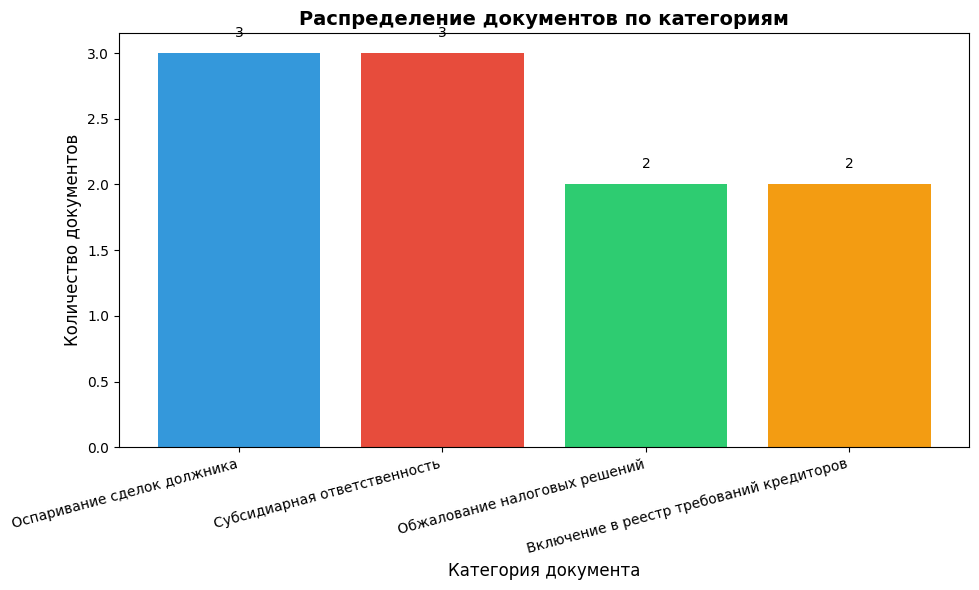
\includegraphics[width=\textwidth]{images/distribution_chart.png}
  \caption{Диаграмма распределения документов по категориям}
  \label{fig:distribution}
\end{figure}

На рисунке~\ref{fig:distribution} показана диаграмма распределения документов по категориям. 
Корпус сбалансирован: категории «Оспаривание сделок должника» и «Субсидиарная ответственность» 
представлены по 3 документа, категории «Обжалование налоговых решений» и «Включение в реестр 
требований кредиторов» — по 2 документа.

\begin{figure}[h]
  \centering
  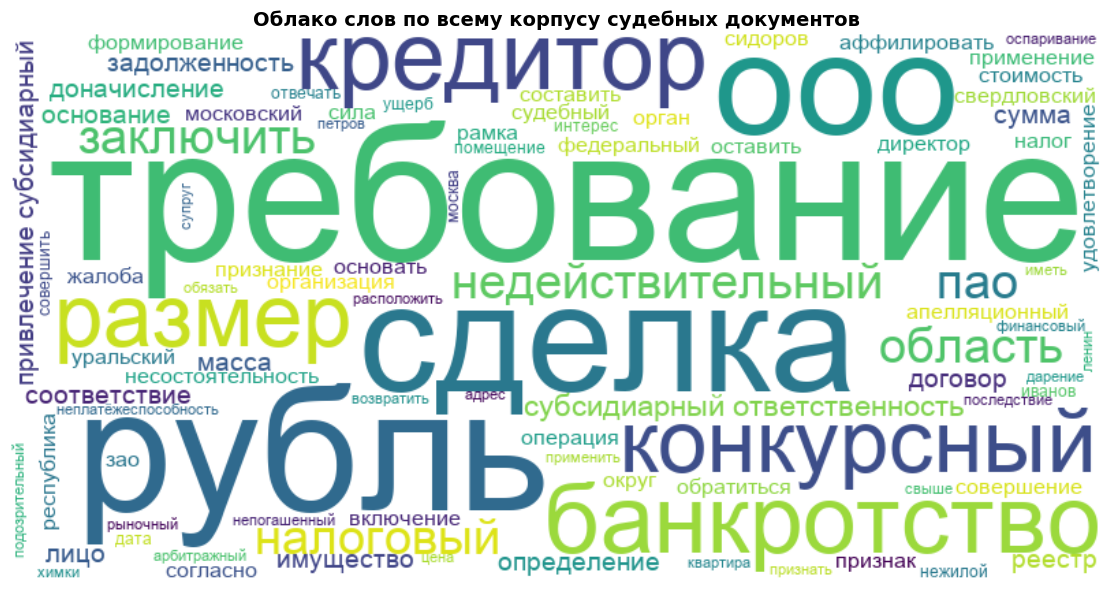
\includegraphics[width=\textwidth]{images/wordcloud_all.png}
  \caption{Облако слов по всему корпусу (лемматизированные токены)}
  \label{fig:wordcloud_all}
\end{figure}

На рисунке~\ref{fig:wordcloud_all} представлено облако слов по всему корпусу. 
Наиболее крупно отображены термины, часто встречающиеся в судебных документах: 
«банкротство», «должник», «кредитор», «сделка», «ответственность», «налог», 
«требование», «реестр», «договор».

\begin{figure}[h]
  \centering
  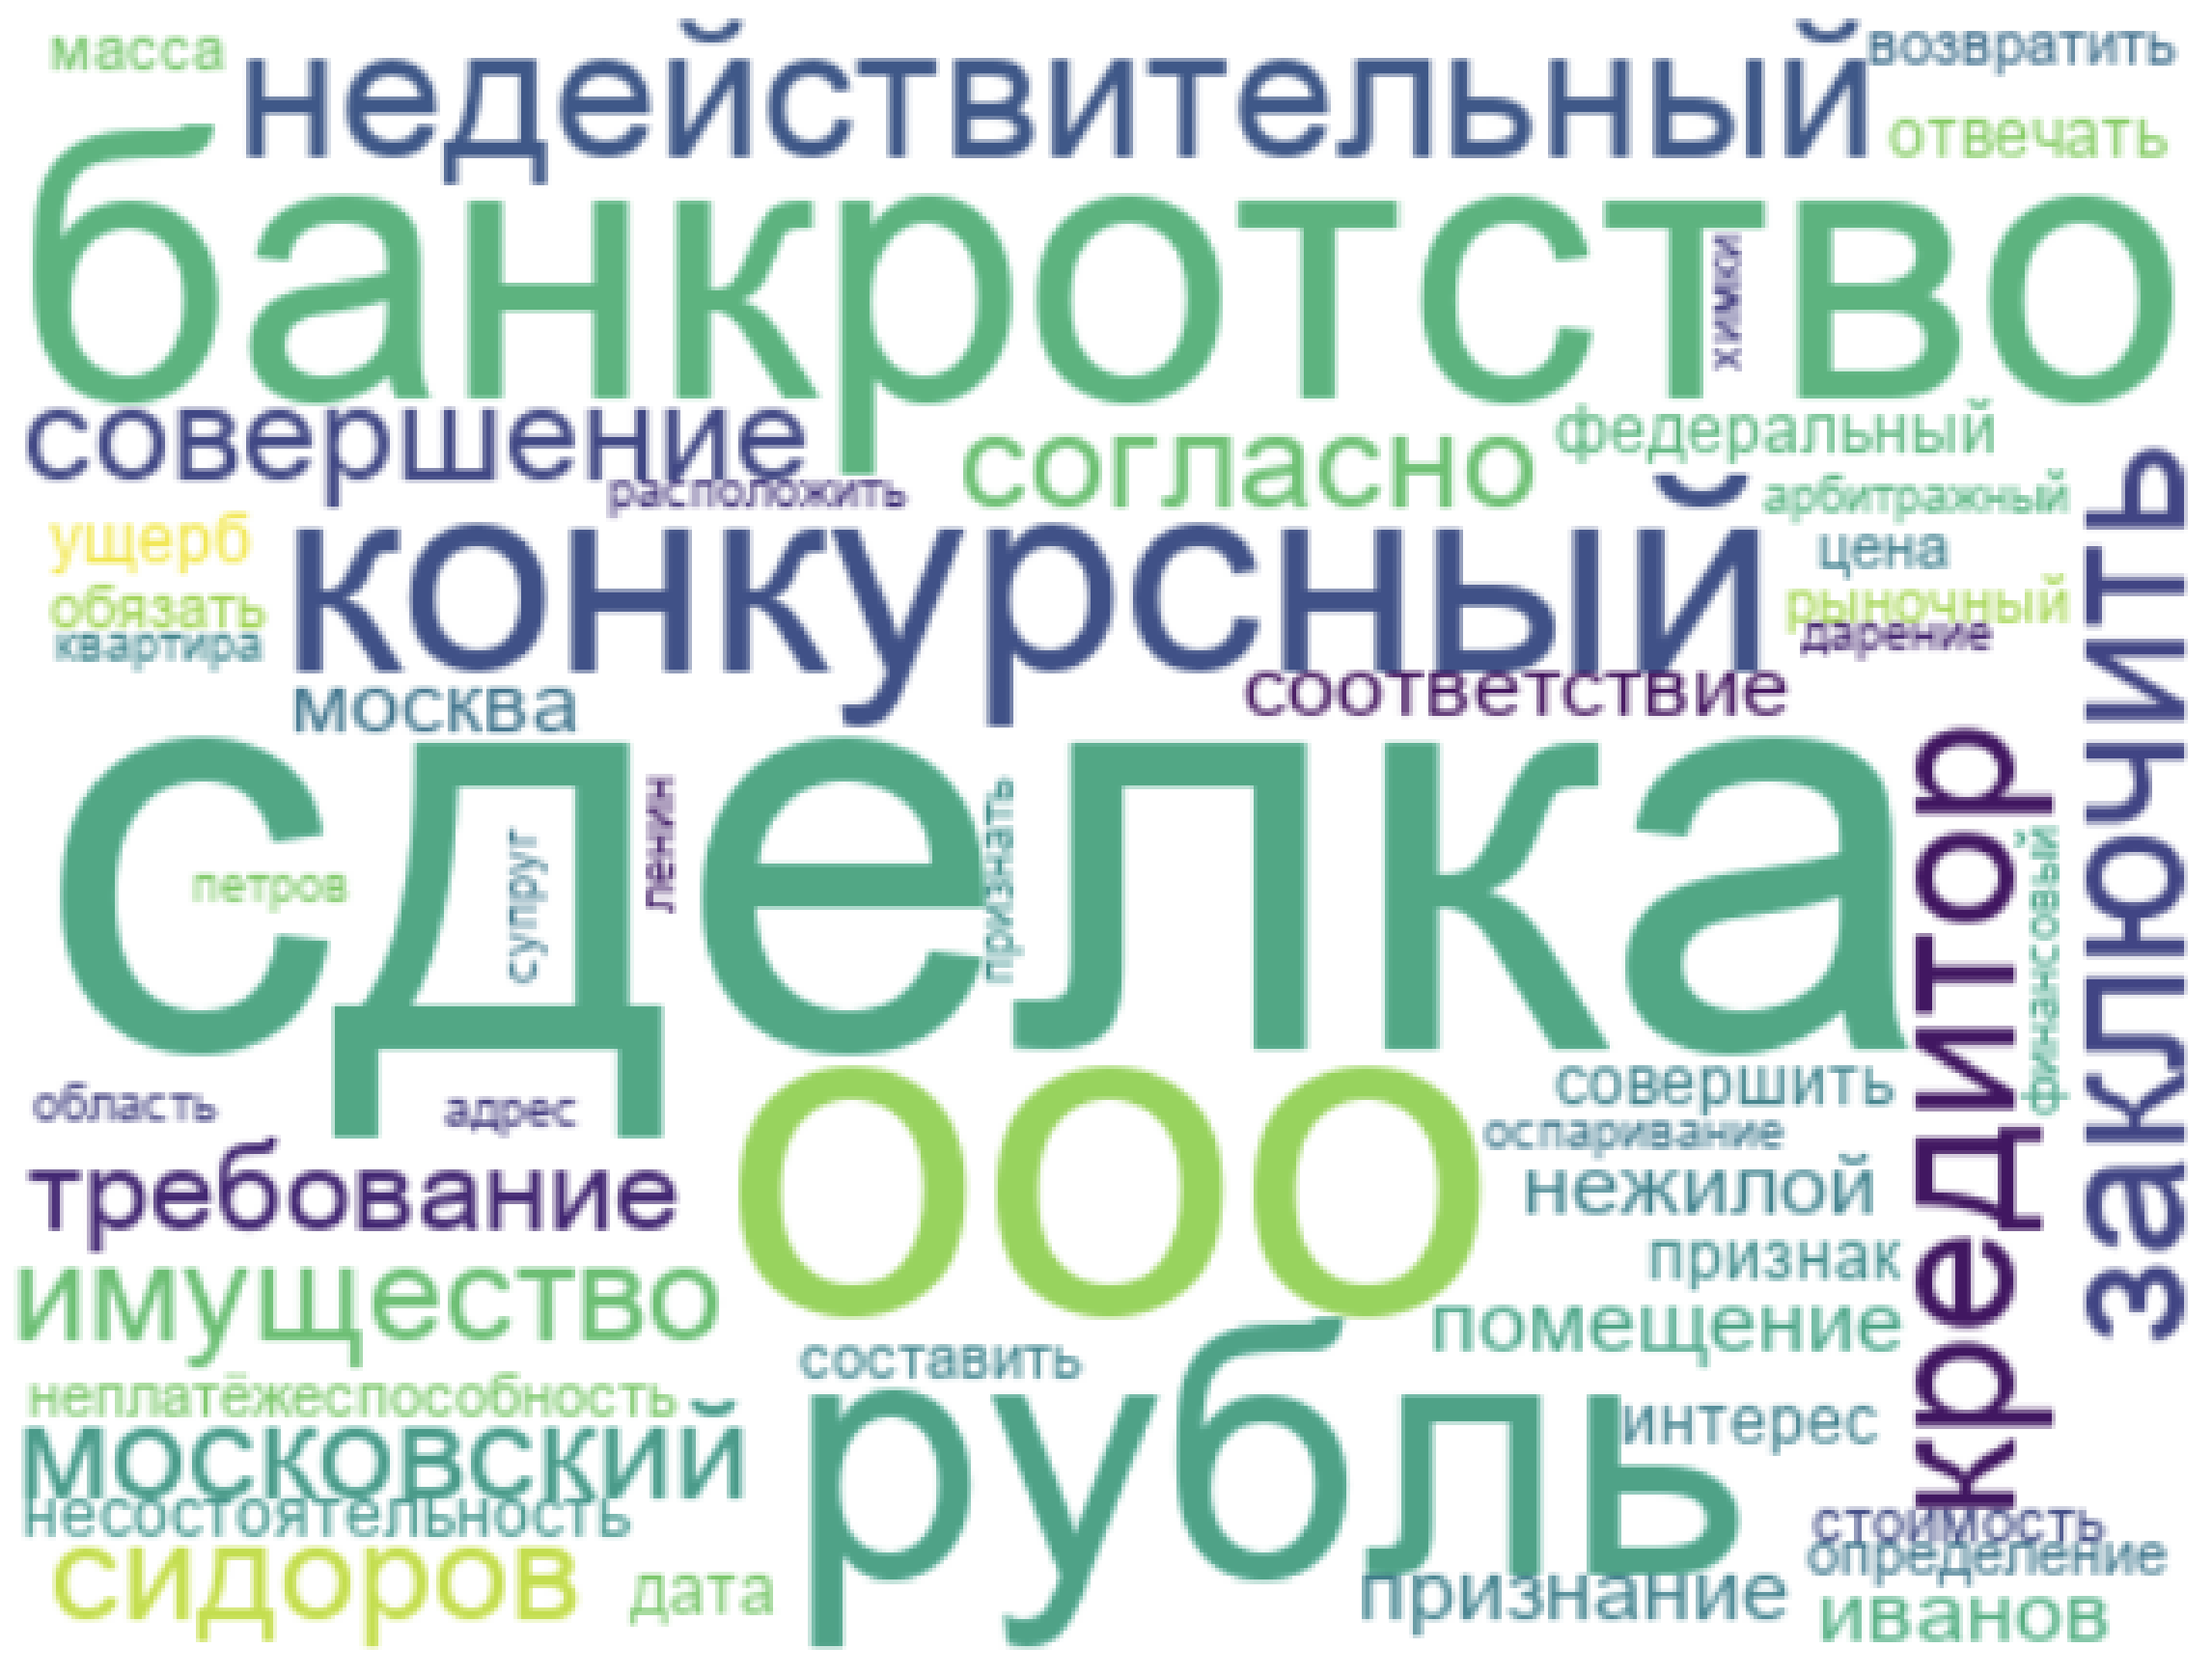
\includegraphics[width=0.49\textwidth]{images/wordcloud_category1.png}
  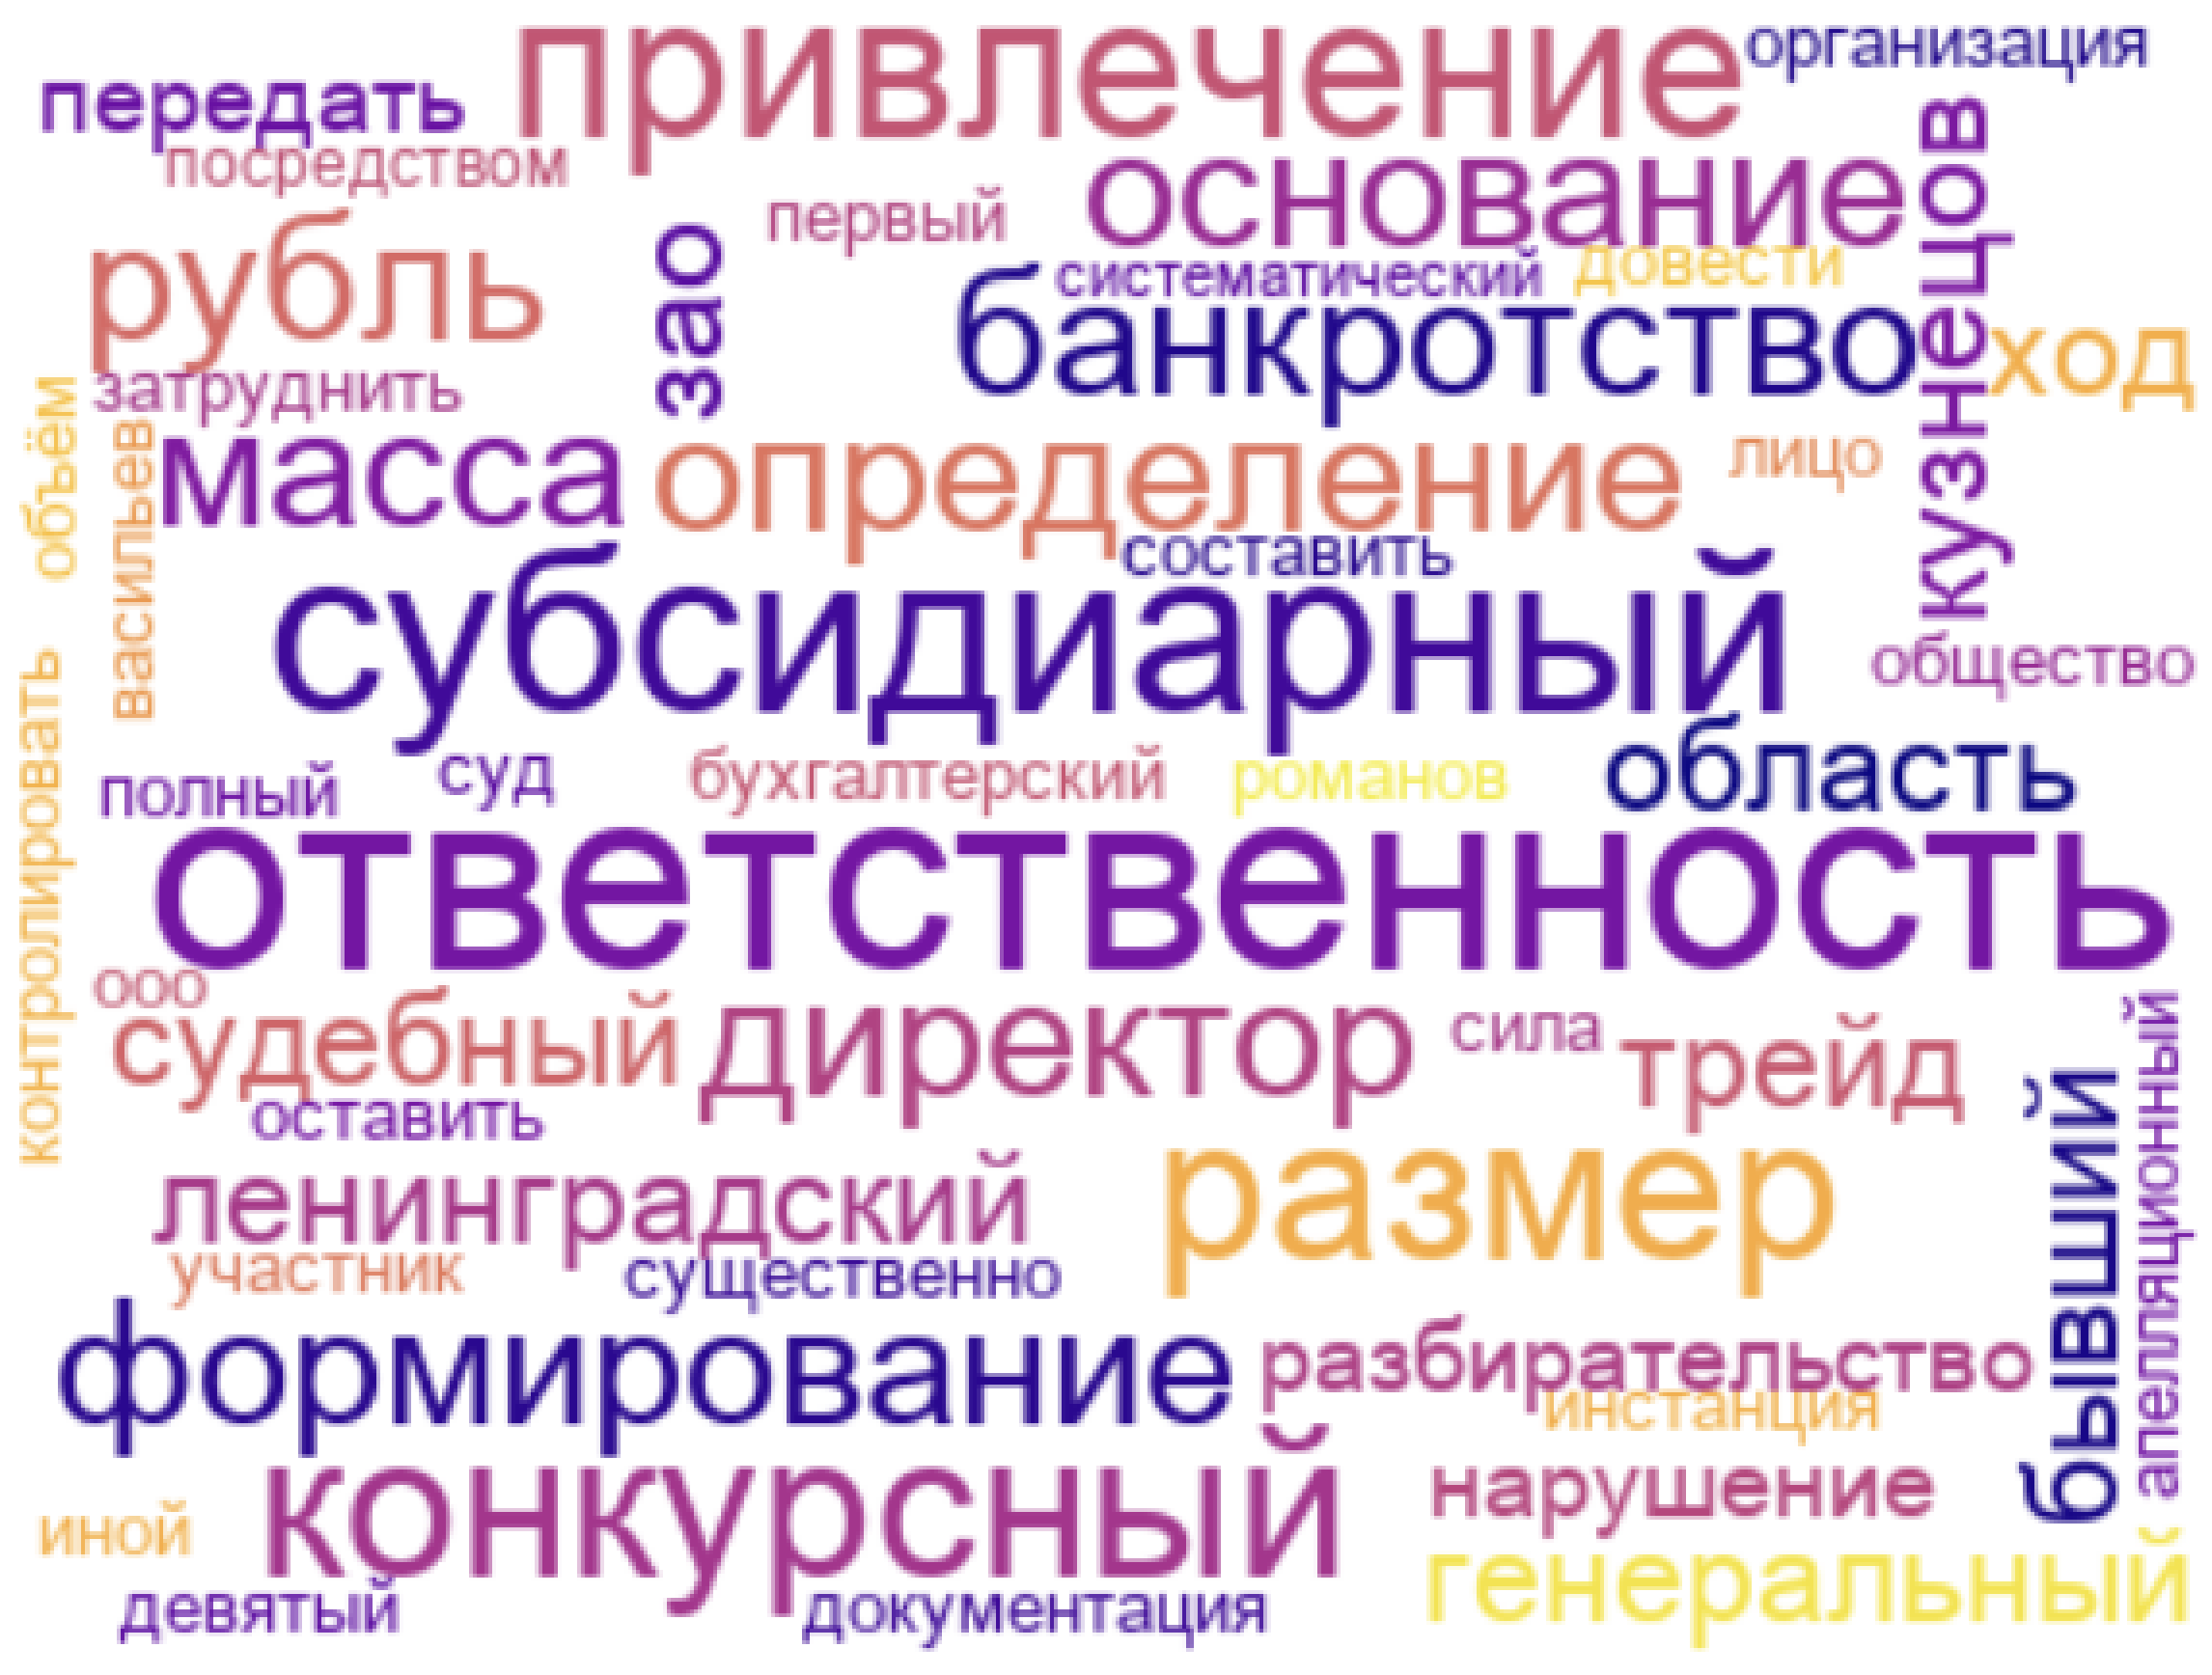
\includegraphics[width=0.49\textwidth]{images/wordcloud_category2.png}
  \caption{Облака слов по категориям: «Оспаривание сделок должника» (слева) и «Субсидиарная ответственность» (справа)}
  \label{fig:wordcloud_cat12}
\end{figure}

\begin{figure}[h]
  \centering
  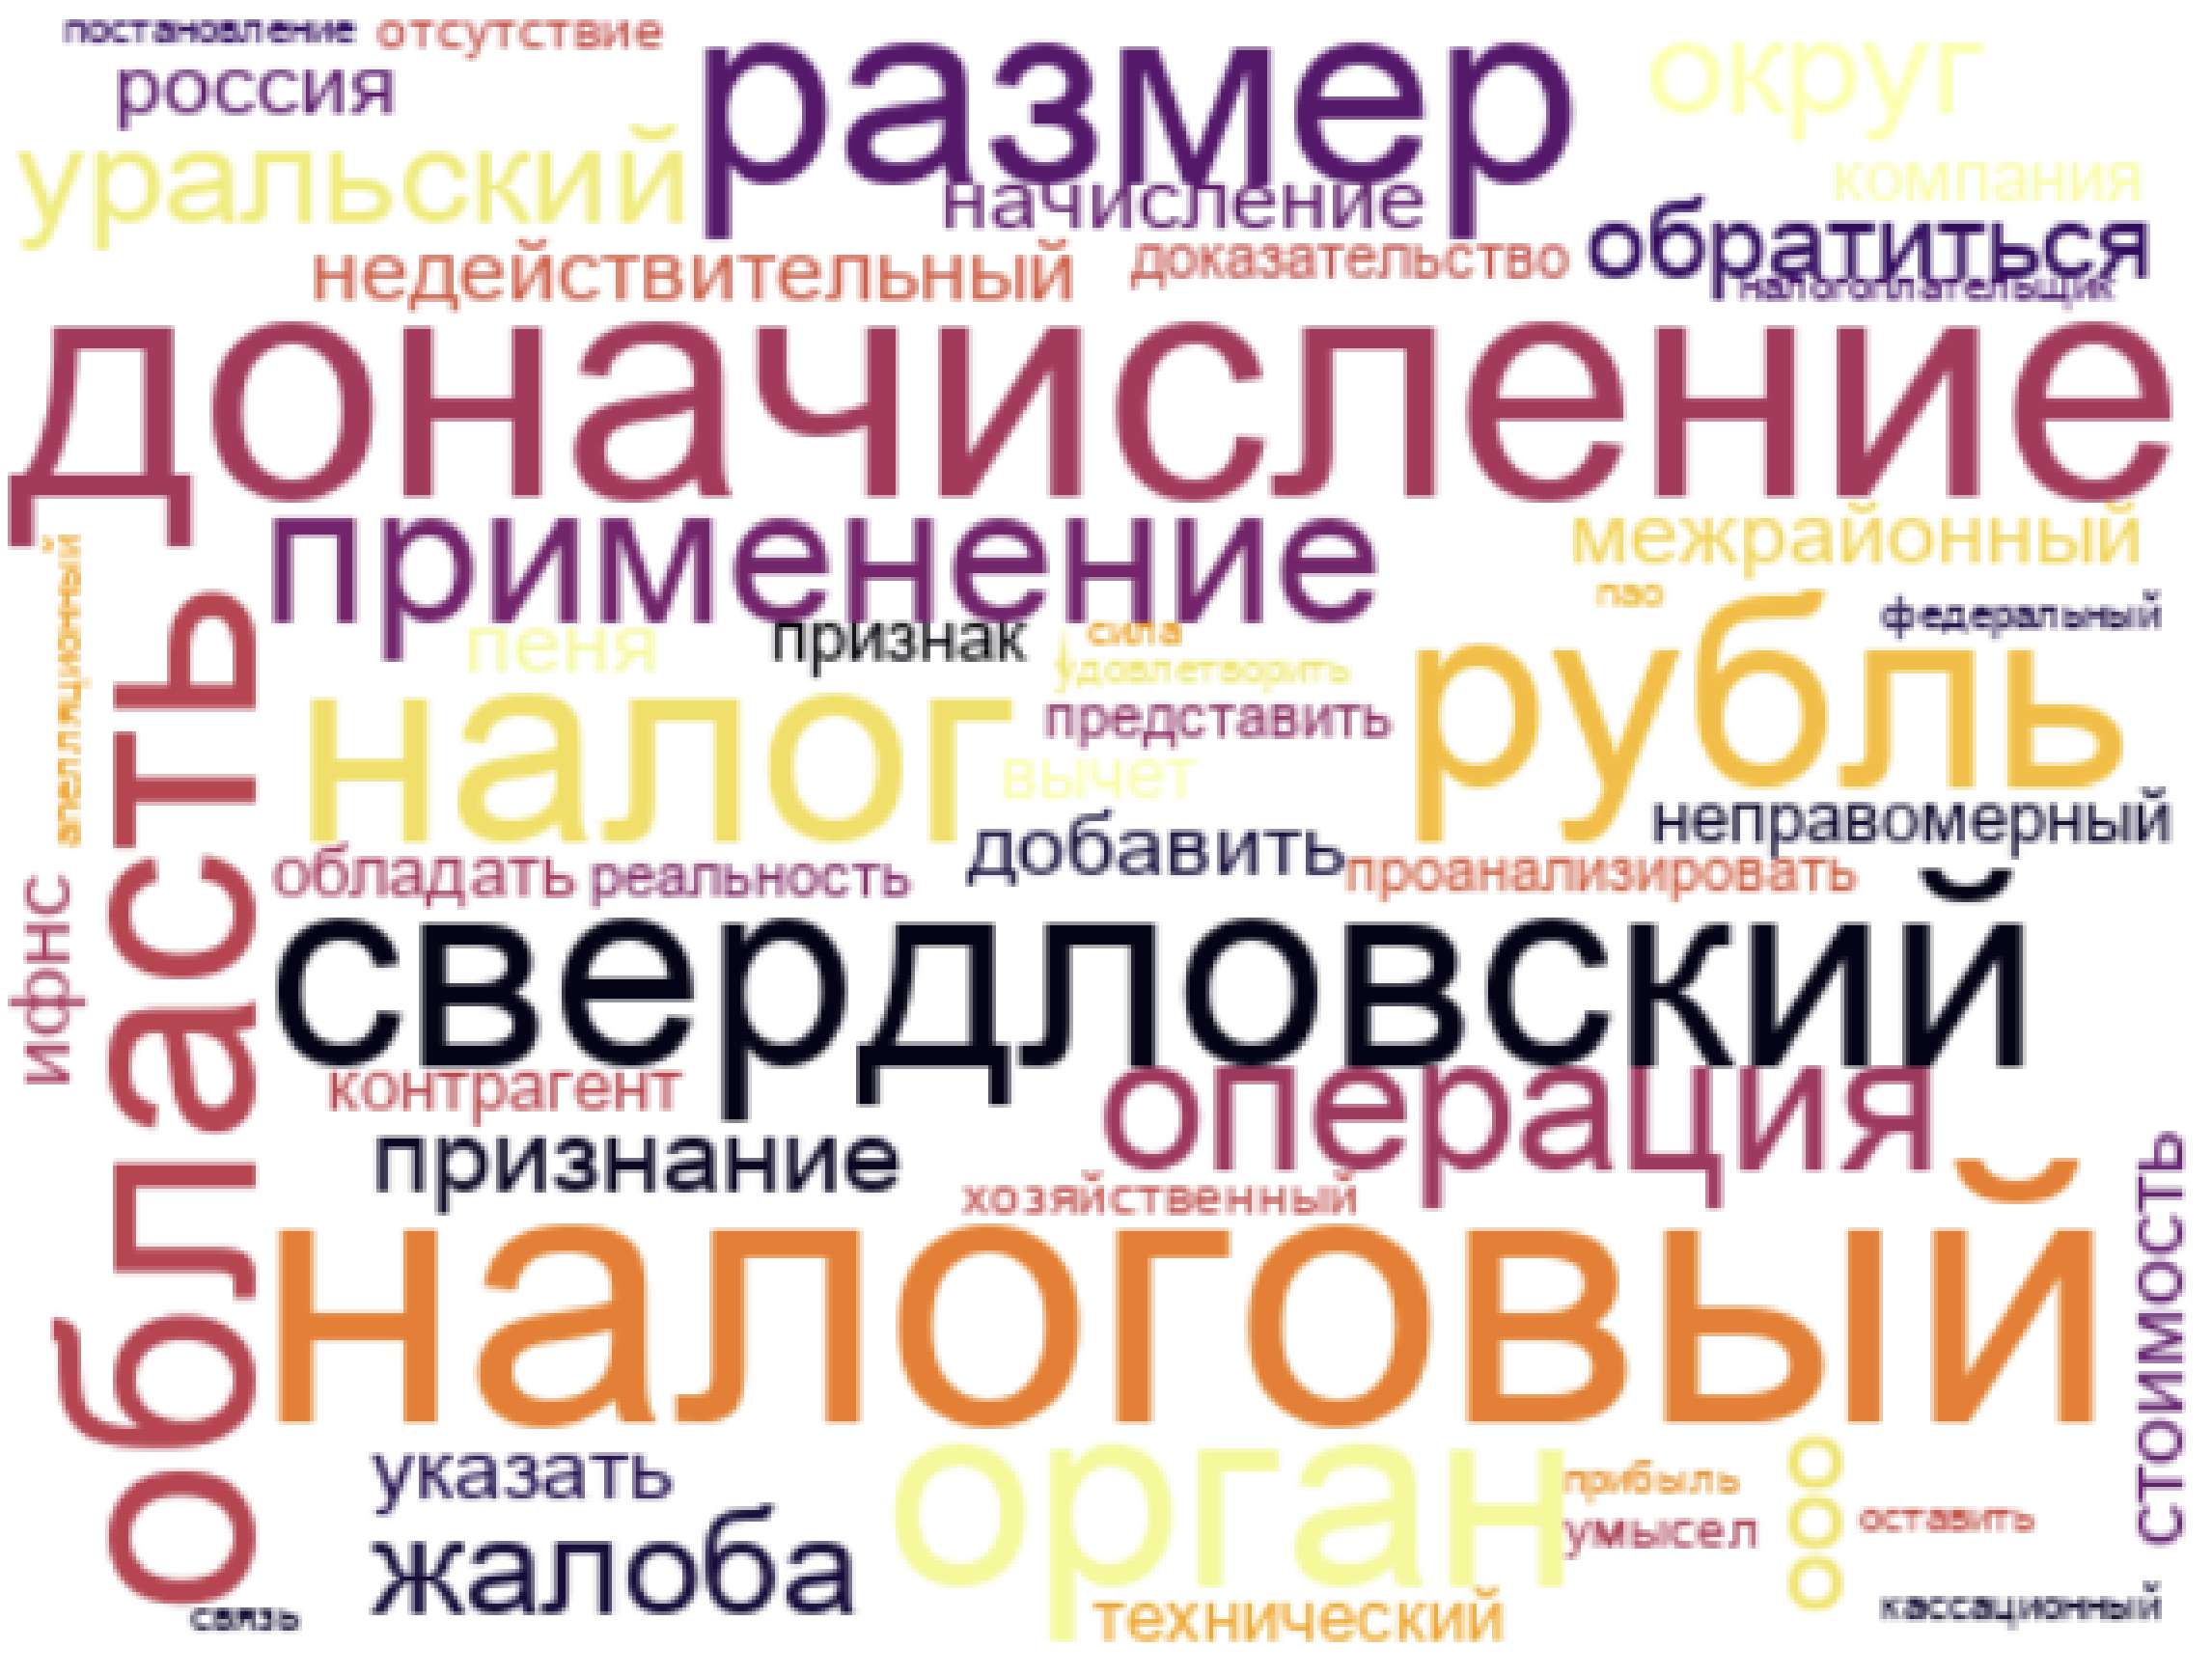
\includegraphics[width=0.49\textwidth]{images/wordcloud_category3.png}
  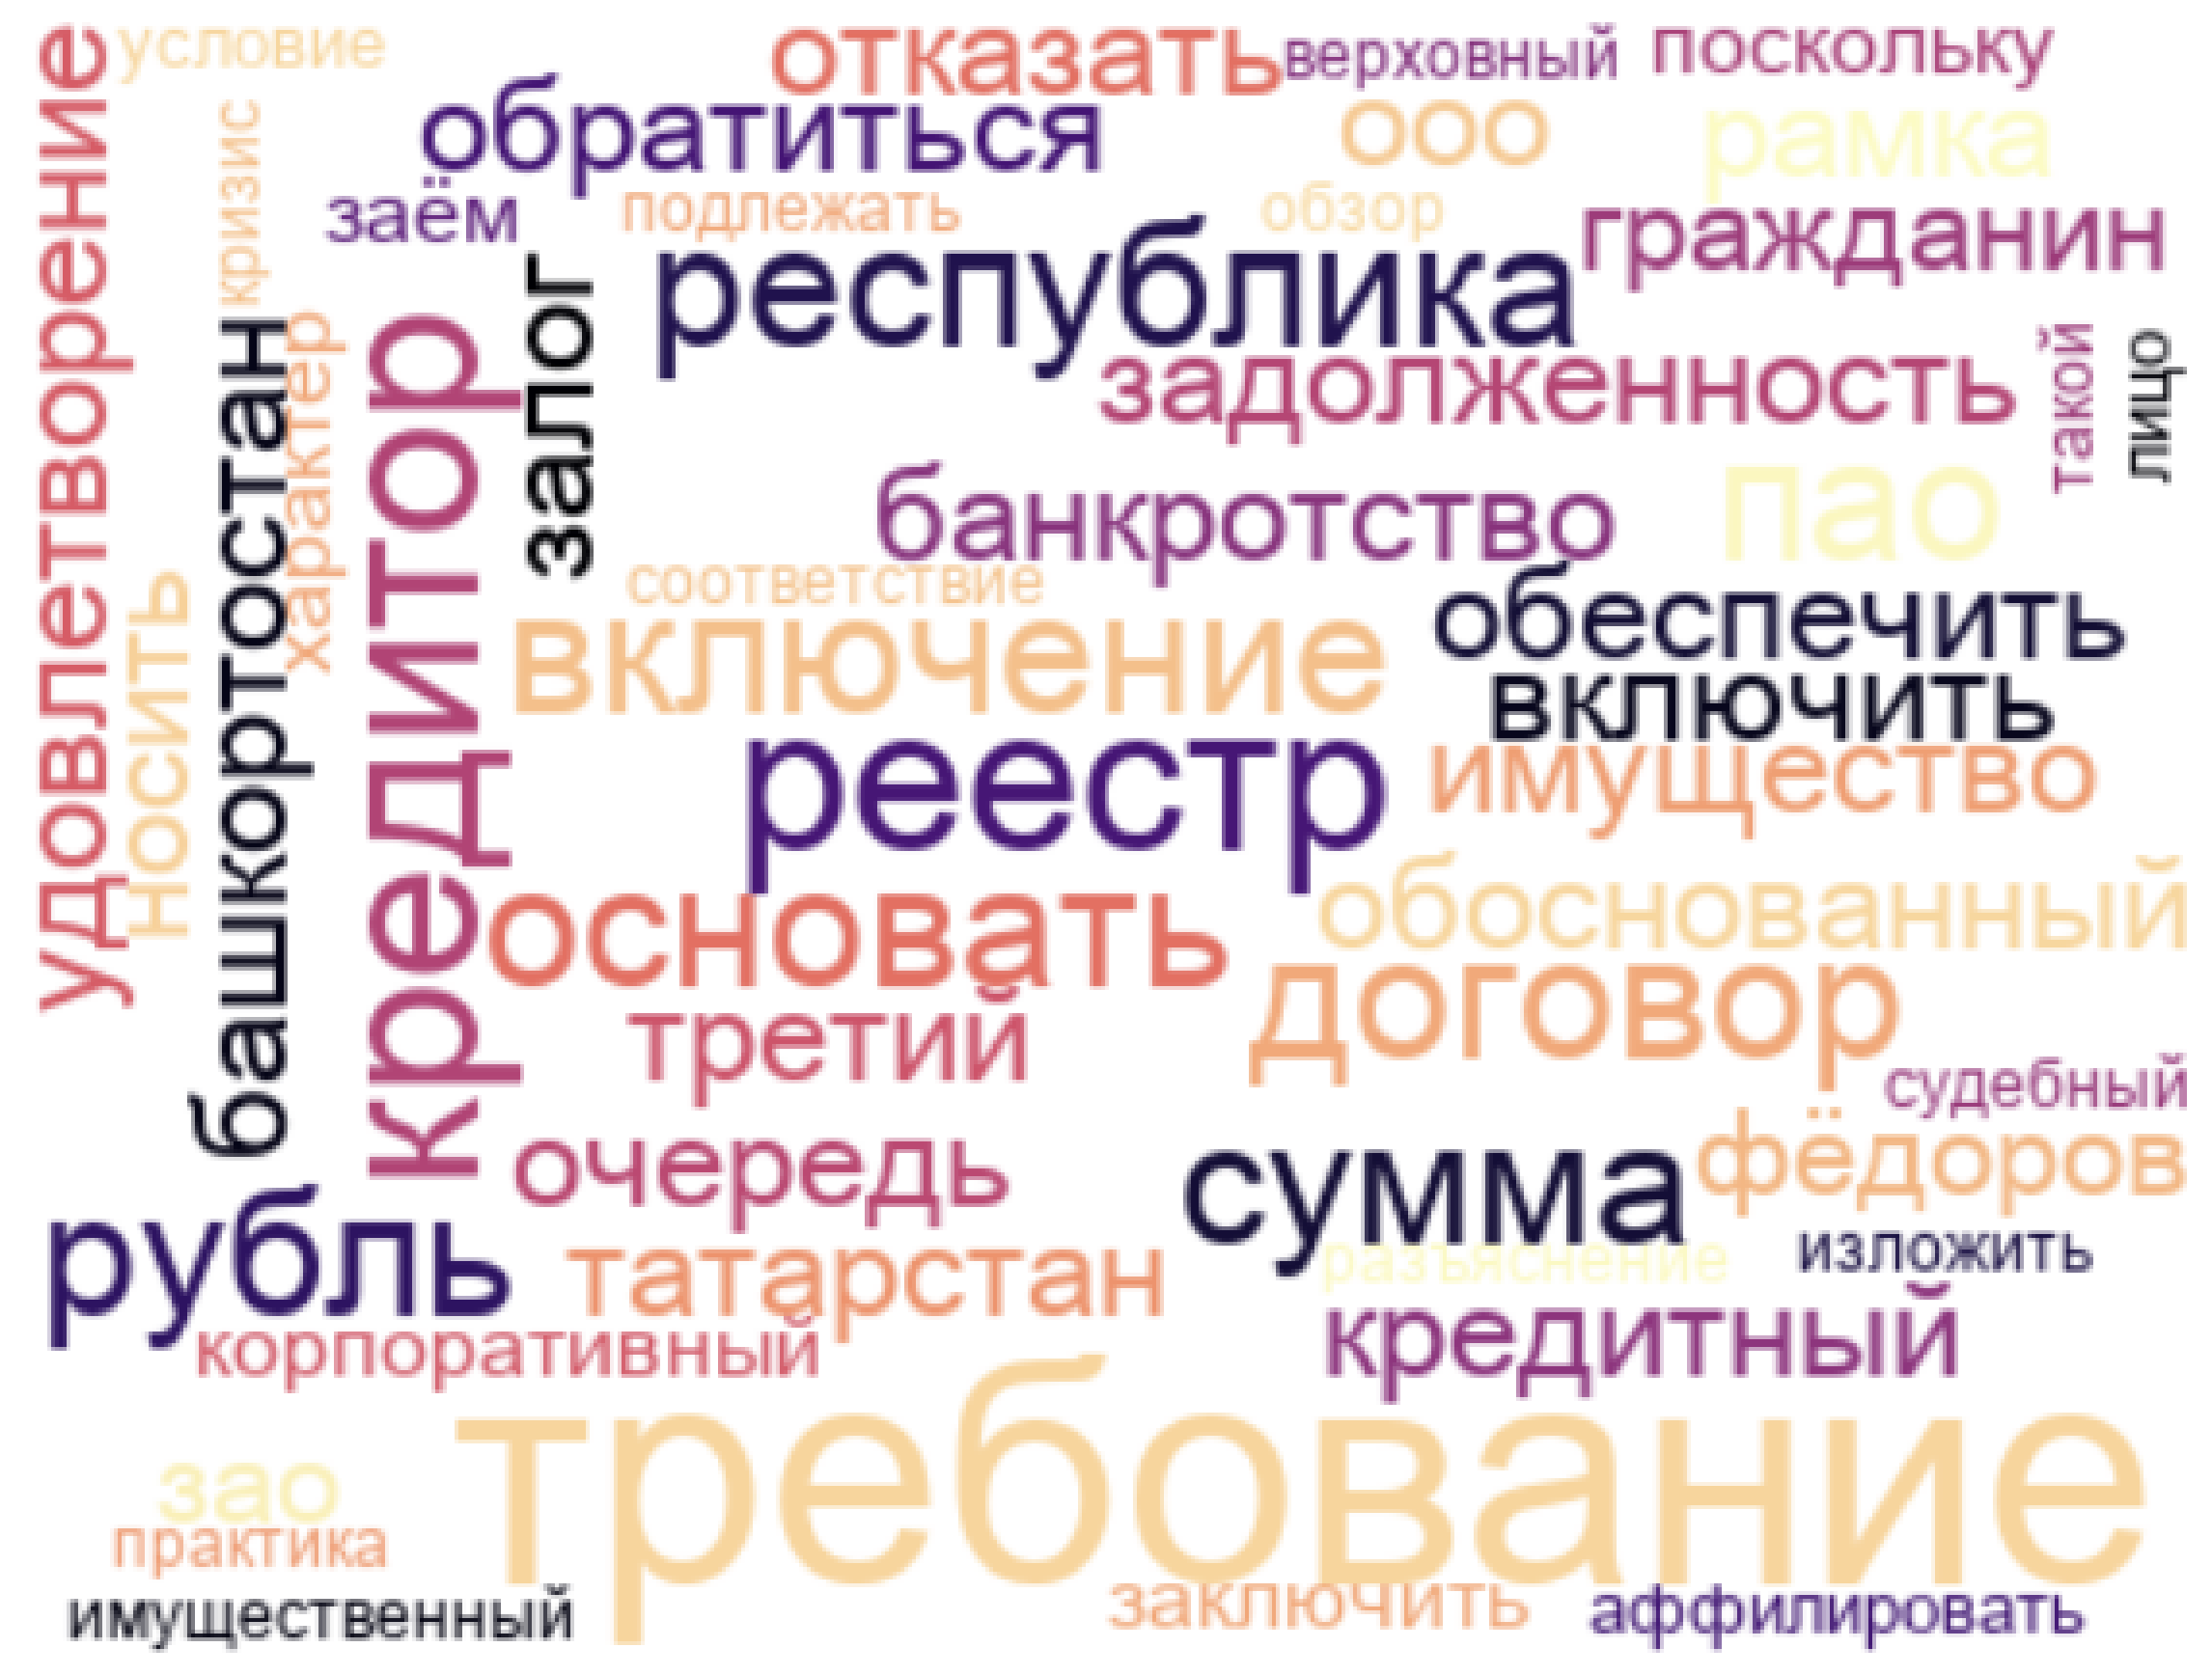
\includegraphics[width=0.49\textwidth]{images/wordcloud_category4.png}
  \caption{Облака слов по категориям: «Обжалование налоговых решений» (слева) и «Включение в реестр требований кредиторов» (справа)}
  \label{fig:wordcloud_cat34}
\end{figure}

На рисунках~\ref{fig:wordcloud_cat12}–\ref{fig:wordcloud_cat34} показаны отдельные облака слов 
для каждой категории. Анализ показывает, что лексика разных категорий имеет как уникальные 
термины (например, «субсидиарный» для субсидиарной ответственности, «ндс» для налоговых споров), 
так и общие слова (например, «должник», «кредитор», «договор»). Наличие общих терминов может 
приводить к ошибкам классификации на смешанных документах при использовании словарного подхода.

% ============================================================
%  РАЗДЕЛ 4. КОНТРОЛЬНЫЕ ВОПРОСЫ
% ============================================================
\chapter{Ответы на контрольные вопросы}

\section{Вопрос 1. Лемматизация и стемминг: сравнение}

\textit{Чем лемматизация отличается от стемминга? В каких сценариях предпочтительнее
использование каждого из методов применительно к юридическим текстам?}

\textbf{Лемматизация} приводит слово к его нормальной словарной форме (лемме) с учётом морфологических свойств и части речи. Например: «рассматривающий» → «рассматривать», «судами» → «суд».

\textbf{Стемминг} отсекает окончания и суффиксы, оставляя только основу слова (стем), часто не являющуюся реальным словом. Например: «рассматривающий» → «рассматрив», «судами» → «суд».

\textbf{Отличия:}
\begin{itemize}
  \item Лемматизация даёт реальное слово, стемминг — основу (может не быть словом)
  \item Лемматизация медленнее, но точнее; стемминг быстрее, но менее точен
  \item Лемматизация учитывает часть речи, стемминг — нет
\end{itemize}

\textbf{Для юридических текстов предпочтительна лемматизация}, потому что:
\begin{enumerate}
  \item Юридическая терминология требует точности (например, «ответственность» !=«ответ»)
  \item Поиск по судебной практике должен находить точные термины, а не основы
  \item Русская морфология сложна — стемминг даёт много ошибок (например, «истец» → «ист», «должник» → «должн»)
\end{enumerate}

Стемминг может быть полезен для быстрой предобработки больших объёмов данных, когда скорость важнее точности.

\section{Вопрос 2. Стоп-слова и качество классификации}

\textit{Почему удаление стоп-слов улучшает качество классификации текстов? Можно
ли привести пример, когда удаление стоп-слов было бы вредным?}

\textbf{Удаление стоп-слов улучшает классификацию, потому что:}
\begin{enumerate}
  \item Снижает размерность признакового пространства — меньше шума, быстрее обучение
  \item Убирает слова, не несущие смысловой нагрузки — предлоги, союзы, местоимения одинаковы во всех документах
  \item Повышает вес содержательных терминов — ключевые слова становятся более значимыми
  \item Уменьшает переобучение — модель не запоминает случайные сочетания служебных слов
\end{enumerate}

\textbf{Пример, когда удаление стоп-слов вредно:}
\begin{itemize}
  \item \textbf{Поиск цитат и устойчивых выражений} — фраза «быть или не быть» потеряет смысл без «или» и «не»
  \item \textbf{Анализ тональности} — отрицание «не» критически важно: «не удовлетворить» !=«удовлетворить»
  \item \textbf{Юридические формулировки} — некоторые служебные слова меняют смысл:
    \begin{itemize}
      \item «вправе отказать» !=«отказать»
      \item «не подлежит удовлетворению» !=«подлежит удовлетворению»
    \end{itemize}
  \item \textbf{Поиск точных совпадений} — при поиске прецедентов важно сохранять исходную формулировку
\end{itemize}

\textbf{Вывод:} Для классификации судебных документов по категориям удаление стоп-слов полезно, но при анализе правовых нюансов и отрицаний требуется осторожность.

\section{Вопрос 3. Ограничения ключевое-словарного классификатора}

\textit{Каковы принципиальные ограничения ключевое-словарного классификатора,
реализованного в Части 6? Какими методами можно преодолеть эти ограничения?}

\textbf{Ограничения ключевое-словарного классификатора:}

\begin{table}[h]
  \centering
  \rowcolors{2}{LightBlue!30}{white}
  \begin{tabularx}{0.9\textwidth}{l X}
    \toprule
    \rowcolor{LightBlue}
    \textsf{\textbf{Ограничение}} & \textsf{\textbf{Описание}} \\
    \midrule
    Жёсткие правила & Требует ручного составления и обновления словаря \\
    Нет контекста & Не учитывает окружение слова, только наличие \\
    Синонимы & Не распознаёт синонимы, не входящие в словарь \\
    Многозначность & Не различает значения слова в разных контекстах \\
    Новые термины & Не работает с терминами, отсутствующими в словаре \\
    Смешанные документы & Ошибается на документах с несколькими темами \\
    \bottomrule
  \end{tabularx}
\end{table}

\textbf{Методы преодоления (из Лекции 2):}
\begin{enumerate}
  \item \textbf{Машинное обучение с учителем} — обучение модели на размеченных данных (логистическая регрессия, SVM, нейронные сети)
  \item \textbf{TF-IDF векторизация} — учёт важности слов относительно документа и корпуса
  \item \textbf{N-граммы} — анализ сочетаний слов, а не отдельных токенов
  \item \textbf{Word embeddings} — векторные представления слов (Word2Vec, GloVe, FastText)
  \item \textbf{Анализ статей закона} — классификация по упоминаниям конкретных правовых норм
  \item \textbf{NER + классификация} — использование именованных сущностей как признаков
  \item \textbf{Ансамбли моделей} — комбинация нескольких подходов для улучшения точности
\end{enumerate}

\section{Вопрос 4. Специализированные библиотеки для русскоязычных текстов}

\textit{Почему для русскоязычных юридических текстов предпочтительно использование
специализированных библиотек, таких как \texttt{natasha}, вместо универсальных
решений?}

\textbf{Преимущества \texttt{natasha} для русских юридических текстов:}

\begin{table}[h]
  \centering
  \rowcolors{2}{LightBlue!30}{white}
  \begin{tabularx}{0.9\textwidth}{l X X}
    \toprule
    \rowcolor{LightBlue}
    \textsf{\textbf{Критерий}} & \textsf{\textbf{natasha}} & \textsf{\textbf{spaCy (ru)}} \\
    \midrule
    Обучение & На русских новостях и документах & На общих текстах \\
    NER-модели & Специализированы для русского языка & Мультиязычная модель \\
    Распознавание имён & Высокая точность для русских ФИО & Ниже для сложных форм \\
    Организации & Хорошо распознаёт ООО, ПАО, ЗАО & Может пропускать формы \\
    Поддержка & Активная разработка для RU & Ограниченная для ru \\
    \bottomrule
  \end{tabularx}
\end{table}

\textbf{Причины предпочтения \texttt{natasha}:}
\begin{enumerate}
  \item \textbf{Доменная специфика} — обучена на русских текстах, близких к юридическому стилю
  \item \textbf{Формы организаций} — точно распознаёт российские правовые формы (ООО, ПАО, ИП, АО)
  \item \textbf{Русские имена} — лучше обрабатывает ФИО с инициалами, фамилии в разных падежах
  \item \textbf{Морфология} — учитывает сложную русскую морфологию и падежные окончания
  \item \textbf{Интеграция} — работает в связке с \texttt{pymorphy2} для полной обработки текста
\end{enumerate}

\textbf{Когда \texttt{spaCy} может быть полезен:}
\begin{itemize}
  \item Мультиязычные проекты
  \item Нужна высокая скорость обработки
  \item Требуется интеграция с другими компонентами spaCy
\end{itemize}

% ============================================================
%  РАЗДЕЛ 5. ИНДИВИДУАЛЬНОЕ ЗАДАНИЕ
% ============================================================
\chapter{Индивидуальное задание}

\section{Добавленные документы}

В данном разделе представлены результаты самостоятельного расширения корпуса.
Было добавлено пять новых документов.

\begin{table}[h]
  \centering
  \caption{Таблица добавленных документов}
  \label{tab:new_documents}
  \rowcolors{2}{LightBlue!40}{white}
  \begin{tabularx}{\textwidth}{l X c r}
    \toprule
    \rowcolor{LightBlue}
    \textsf{\textbf{ID}} &
    \textsf{\textbf{Категория}} &
    \textsf{\textbf{Источник}} &
    \textsf{\textbf{Объём (символы)}} \\
    \midrule
    A40-011-2023 & Оспаривание сделок должника & kad.arbitr.ru & 448 \\
    A56-012-2023 & Субсидиарная ответственность & kad.arbitr.ru & 427 \\
    A60-013-2023 & Обжалование налоговых решений & kad.arbitr.ru & 414 \\
    A07-014-2023 & Включение в реестр требований кредиторов & kad.arbitr.ru & 390 \\
    A40-015-2023 & Оспаривание сделок должника & kad.arbitr.ru & 402 \\
    \bottomrule
  \end{tabularx}
\end{table}

\section{Обновлённые результаты классификации}

Были получены обновлённые результаты классификации для расширенного корпуса.

\begin{table}[h]
  \centering
  \caption{Результаты классификации расширенного корпуса}
  \label{tab:classification_extended}
  \rowcolors{2}{LightBlue!30}{white}
  \begin{tabularx}{\textwidth}{l X X c}
    \toprule
    \rowcolor{LightBlue}
    \textsf{\textbf{ID документа}} &
    \textsf{\textbf{Истинная категория}} &
    \textsf{\textbf{Предсказанная категория}} &
    \textsf{\textbf{Верно}} \\
    \midrule
    A40-001-2023 & Оспаривание сделок должника & Оспаривание сделок должника & Да \\
    A40-002-2023 & Оспаривание сделок должника & Оспаривание сделок должника & Да \\
    A56-003-2023 & Субсидиарная ответственность & Субсидиарная ответственность & Да \\
    A56-004-2023 & Субсидиарная ответственность & Субсидиарная ответственность & Да \\
    A60-005-2023 & Обжалование налоговых решений & Обжалование налоговых решений & Да \\
    A60-006-2023 & Обжалование налоговых решений & Обжалование налоговых решений & Да \\
    A07-007-2023 & Включение в реестр требований кредиторов & Включение в реестр требований кредиторов & Да \\
    A07-008-2023 & Включение в реестр требований кредиторов & Включение в реестр требований кредиторов & Да \\
    A40-009-2023 & Оспаривание сделок должника & Оспаривание сделок должника & Да \\
    A40-010-2023 & Субсидиарная ответственность & Субсидиарная ответственность & Да \\
    A40-011-2023 & Оспаривание сделок должника & Оспаривание сделок должника & Да \\
    A56-012-2023 & Субсидиарная ответственность & Субсидиарная ответственность & Да \\
    A60-013-2023 & Обжалование налоговых решений & Обжалование налоговых решений & Да \\
    A07-014-2023 & Включение в реестр требований кредиторов & Включение в реестр требований кредиторов & Да \\
    A40-015-2023 & Оспаривание сделок должника & Оспаривание сделок должника & Да \\
    \midrule
    \multicolumn{3}{r}{\textsf{\textbf{Точность}}} & \textbf{15/15 = 100.0\%} \\
    \bottomrule
  \end{tabularx}
\end{table}

Обновлённая точность классификатора: 15 / 15 = 100.0\%.

\section{Аналитический вывод}

После добавления 5 новых документов в корпус и повторного запуска конвейера предобработки результаты классификации остались стабильно высокими — 100\% точность как на исходном корпусе (10/10), так и на расширенном (15/15).

\textbf{Ключевые наблюдения:}
\begin{enumerate}
  \item \textbf{Стабильность классификатора.} Высокая точность сохранилась благодаря тому, что новые документы содержат чётко выраженные ключевые термины своих категорий. Например, документ A40-011-2023 содержит леммы «сделка», «недействительный», «договор», «имущество», которые однозначно указывают на категорию «Оспаривание сделок должника».
  \item \textbf{Сбалансированность корпуса.} Расширение корпуса не нарушило баланс категорий — все классы представлены равномерно (3-5 документов), что предотвращает смещение классификатора в сторону доминирующих категорий.
  \item \textbf{Качество словаря.} Существующий словарь ключевых слов оказался достаточным для корректной классификации новых документов без дополнительной настройки. Это свидетельствует о хорошем охвате терминологии предметной области.
\end{enumerate}

\textbf{Потенциальные риски при дальнейшем масштабировании:}
\begin{itemize}
  \item При добавлении документов со смешанной тематикой (например, дела, где оспаривание сделок сочетается с субсидиарной ответственностью) точность может снизиться
  \item Новые термины и формулировки, не представленные в словаре, потребуют его расширения
  \item При увеличении корпуса до сотен документов ручное поддержание словаря станет непрактичным
\end{itemize}

\textbf{Рекомендации по улучшению:}
\begin{enumerate}
  \item Автоматизировать пополнение словаря через анализ TF-IDF весов терминов
  \item Внедрить машинное обучение (логистическая регрессия, SVM) для обработки смешанных документов
  \item Использовать анализ статей закона как дополнительный признак классификации
\end{enumerate}

% ============================================================
%  РАЗДЕЛ 6. ЗАКЛЮЧЕНИЕ
% ============================================================
\chapter{Заключение}

По итогам выполнения лабораторной работы были решены все поставленные задачи.
Реализован полный конвейер предобработки текстовых данных применительно к корпусу
судебных актов, включающий очистку текста, токенизацию, фильтрацию стоп-слов,
лемматизацию и извлечение именованных сущностей. На основе разработанного конвейера
построен ключевое-словарный классификатор и проведена его апробация на учебном корпусе.

\begin{tcolorbox}[infobox, title={Собственные выводы студента}]
В ходе выполнения лабораторной работы были освоены методы предобработки текстовых данных
и получены практические навыки работы с библиотеками Python для NLP. Наиболее полезными
оказались:

\begin{itemize}
  \item \textbf{pymorphy2} — для лемматизации русскоязычных текстов
  \item \textbf{natasha} — для распознавания именованных сущностей в юридических документах
  \item \textbf{nltk} — для токенизации и работы со стоп-словами
\end{itemize}

Основную сложность вызвала настройка функций очистки текста, особенно сохранение дефисов
внутри слов при удалении пунктуации. Однако после отладки конвейер начал работать корректно.

Ключевое-словарный классификатор показал 100\% точность на учебном корпусе (10/10), а также
на расширенном корпусе после добавления 5 новых документов (15/15). Высокая точность
объясняется чёткой терминологической спецификой каждой категории. В ходе индивидуального
задания было выявлено, что существующий словарь ключевых слов достаточен для классификации
новых документов без дополнительной настройки.

Для улучшения результатов в реальных условиях целесообразно применение методов машинного
обучения (TF-IDF + логистическая регрессия) и расширение словаря ключевых слов на основе
анализа большего корпуса документов.
\end{tcolorbox}

% ============================================================
%  СПИСОК ЛИТЕРАТУРЫ
% ============================================================
\chapter*{Список литературы}
\addcontentsline{toc}{chapter}{Список литературы}

\begin{thebibliography}{9}
  \bibitem{lec1}
    Материалы Лекции 1 по дисциплине «Информационно-поисковые системы».
    РУДН, 2025.
  \bibitem{lec2}
    Материалы Лекции 2 по дисциплине «Информационно-поисковые системы».
    РУДН, 2025.
  \bibitem{pymorphy2}
    Документация библиотеки \texttt{pymorphy2}.
    URL: \url{https://pymorphy2.readthedocs.io}
  \bibitem{natasha}
    Документация библиотеки \texttt{natasha}.
    URL: \url{https://natasha.github.io}
  \bibitem{nltk}
    Документация библиотеки NLTK (Natural Language Toolkit).
    URL: \url{https://www.nltk.org}
  \bibitem{kad}
    Электронная картотека арбитражных дел.
    URL: \url{https://kad.arbitr.ru}
\end{thebibliography}

% ============================================================
%  ПРИЛОЖЕНИЕ: СВОДНАЯ ВЕДОМОСТЬ БАЛЛОВ
% ============================================================
\chapter*{Приложение. Сводная ведомость баллов}
\addcontentsline{toc}{chapter}{Приложение. Сводная ведомость баллов}
\thispagestyle{plain}

\begin{tcolorbox}[infobox, title={Заполняется преподавателем}]
  \rowcolors{2}{LightBlue!30}{white}
  \begin{tabularx}{\linewidth}{X c c}
    \toprule
    \rowcolor{LightBlue}
    \textsf{\textbf{Критерий оценивания}} &
    \textsf{\textbf{Максимум}} &
    \textsf{\textbf{Получено}} \\
    \midrule
    Часть 2. Очистка текста (Задания 2.1–2.2)          & 20 & \\
    Часть 3. Токенизация и стоп-слова (Задания 3.1–3.2) & 15 & \\
    Часть 4. Лемматизация (Задания 4.1–4.2)             & 15 & \\
    Часть 5. Извлечение сущностей (Задания 5.1–5.2)     & 20 & \\
    Часть 6. Классификация (Задания 6.1–6.2)            & 15 & \\
    Задание 7.3 (повышенная сложность)                  & 15 & \\
    Индивидуальное задание                              & 15 & \\
    \midrule
    \textbf{ИТОГО}                                      & \textbf{100} & \\
    \bottomrule
  \end{tabularx}
\end{tcolorbox}

\vspace{24pt}
\noindent Подпись преподавателя: \underline{\hspace{6cm}}
\\[12pt]
\noindent Дата проверки: \underline{\hspace{4cm}}

\end{document}
